\documentclass[DM,authoryear,toc]{lsstdoc}
% lsstdoc documentation: https://lsst-texmf.lsst.io/lsstdoc.html
\input{meta}

% Package imports go here.
\usepackage{graphicx}

% Local commands go here.

\title{AWS Proof of Concept Project Report}

\author{
Hsin-Fang Chiang,
}

\setDocRef{DMTN-137}
\setDocUpstreamLocation{\url{https://github.com/lsst-dm/dmtn-137}}

\date{\vcsDate}

\setDocAbstract{%
From April to December 2019, team members from LSST-DM, AWS, and HTCondor undertook a proof-of-concept project to do LSST processing on the AWS platform. This document reports the results.
}

% Change history defined here.
% Order: oldest first.
% Fields: VERSION, DATE, DESCRIPTION, OWNER NAME.
% See LPM-51 for version number policy.
\setDocChangeRecord{%
  \addtohist{1}{YYYY-MM-DD}{Unreleased.}{Hsin-Fang Chiang}
}


\begin{document}

% Create the title page.
%\maketitle
% Frequently for a technote we do not want a title page  uncomment this to remove the title page and changelog.
% use \mkshorttitle to remove the extra pages
\mkshorttitle

\section{Background}

In April 2019, LSST DM began a proof of concept project with the AWS and HTCondor teams to explore whether a cloud deployment of the Data Release Production (DRP) is feasible. The execution plan of the project is described in DMTN-114.  In this document we report the results.



\section{Approaches and Strategies}

In executing this PoC we focused on the goal of being able to demonstrate the data processing on the AWS cloud and kept the following strategies in mind.



\begin{enumerate}
\item
Progress in phases.
\end{enumerate}


\section{Architecture Design}

The system design in the end of the PoC is as in the diagram in Figure~\ref{fig:arch}.

\begin{figure}
  \centering
  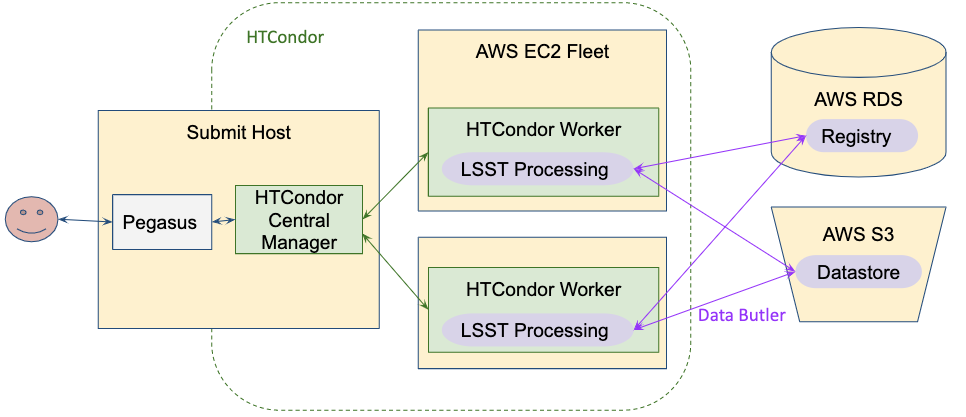
\includegraphics[width=\textwidth]{figures/arch}
  \label{fig:arch}
  \caption{architecture design}
\end{figure}

\subsection{Alternative architecture designs were also discussed in the PoC}

\section{Building AWS support into the Data Butler and lessons learned}

The Data Butler is the overarching data IO abstraction through which all LSST data access is mediated. Datasets are referred to by their unique IDs, or a set of identifying references, which are then resolved through an registry that matches the dataset IDs, or references, to the location, file format and the Python object type of the dataset. The system that persists, reads and potentially modifies the datasets is called the datastore. The Registry almost always backed by an SQL database and the Datastore is usually backed by a shared filesystem. A major focus of AWS POC was to implement, and investigate issues related to, an S3 backed Datastore and a PostgreSQL backed Registry.

Simple Storage Service (S3) is object storage provided by AWS. Unlike the more traditional file systems that manage data as a file hierarchy, or data blocks within sectors and tracts, objet storage manages data as objects. This allows the storage of massive amounts of unstructured data where each object typically includes the data, related metadata and is identified by a globally unique identifier. S3, specifically, promises 99.999999999\% durability as uploading an object to it automatically stores it across multiple systems, thus also ensuring scalability and performance. Related objects are generally stored in the same Buckets for easier administrative purposes. Access, read, write, delete and other atomical units of action on the objects themselves can be allowed or forbidden at the account, bucket or individual object level. Logging is available for all actions on the Bucket level and/or at the individual object granularity. It is also possible to define and issue complex alert conditions on Bucket or object actions which can execute arbitrary actions or workflows.

PostgreSQL is one of the most popular open source relational database systems available. The choice to go with PostgreSQL was based on the fact that it's a very popular and well supported open source software that suffers from no additional licensing fees usually associated with proprietary software. Relational Database Service (RDS) is the AWS cloud service that launches and configures databases with ease. 

At the time the AWS POC Group began generation 3 Butler, the latest implementation of the Data Butler, implemented PosixDatastore, a local or shared filesystem datastore, and a SqliteRegistry. OracleRegistry followed soon after LSST AWS POC group began work. Initialy the focus was on implementing an S3 backed datastore called S3Datastore. The interface between AWS services and LSST Stack would be based on the official AWS SDK called boto3. In March 2019, Dino Bektesevic visited NOAO to work more closely with Tim Jenness, which prooved to be instrumental in implementing the early versions of a new module in the `daf\_butler` called `s3utils`, an `S3Datastore` class, the PosixDatastore equivalent, and a set of appropriate unit tests that demonstrated its functionality and correctness. The unit tests for the datastore utilize the `moto` library which mocks requests and responses sent to AWS services, so that no additional external infrastructure is required to use it. PostgreSqlRegistry class was implemented partially during the visit and completed shortly after the visit. The initial implementation showcasing the required changes to the code was submitted as a Draft Pull Request \href{https://github.com/lsst/daf_butler/pull/147}{PR-147}. 

The tentative implementation revealed issues with how the Data Butler treated Uniform Resource Identifiers, or URIs, which were, at the time, not being handled correctly, as per standards defined in \href{https://tools.ietf.org/html/rfc3986}{FC-3986}, by The Location class. After expansive discussions and an example re-implementation called S3Location to demonstrate the issues, in May 2019 Tim Jenness authored the `ButlerURI` class (\href{https://github.com/lsst/daf_butler/pull/167}{PR-167}) resolving the issues. Major efforts were then invested into refining the newly added code to the level of production quality as well as updating the remaining Gen. 3 Butler to use the updated ButlerURI code instead. Every call to OS functionality had to be generalized to take a URI and from it determine the appropriate operation - a call to OS functionality, a AWS operation or something else. This led changes in Butler, Config, ButlerConfig and YAML Loader classes. These changes made the whole of Data Butler more general and pliable to future changes, such as adding support for other cloud providers. 

Further integration of the S3 backend required a change to Formatter classes to enable data serialization and deserialization to and from bytes. Formatters present interfaces for reading and writing of Python objects to and from files. They are the mechanism underlying how Data Butler is capable of presenting data as science products in the form of Python objects, abstracting away the underlying file types. Modifications were made to JsonFormatter, PickeFormatter, YamlFormatter, PexConfigFormatter and the generic abstract class Formatter. This concluded the last of changes required for S3Datastore integration. After which Jenkins integration tests were run and the S3Datastore and supplemental code was merged to master branch of the `daf\_butler` repository in \href{https://github.com/lsst/daf_butler/pull/179}{PR-179} (the associated Jira ticket is \href{https://jira.lsstcorp.org/browse/DM-13361}{DM-13361}). It became apparent that there are certain similarities that are shared between PosixDatastore and S3Datastore, similarities that would be shared by other future datastore implentations. To reduce code duplication the general datastore code was refactored and reorganized in \href{https://github.com/lsst/daf_butler/pull/187}{PR-187} shortly after. 

PostgreSqlRegistry was not part of this PR. The initial implementation was based on OracleRegistry, due to the similarities between the two, but was re-implemented in terms of the generic SqlRegistry class in July. Problems were caused, for both Oracle and PostgreSQL, by the table naming conventions and additionally, for PostgreSQL, the table views did not conform to the assumptions made. In July the PostgreSqlRegistry was re-implemented in terms of the more general SqlRegistry and a new SQLAlchemy expressions compiler was written, so that table views could be generated correctly. The policy for additional registry implementations was not to accept associated unit tests, as they are dependent on existing outside architecture, meant that checking wheter it worked or not had to be based on manually executing one of the continuous integration tests such as ci\_hsc. I migrated existing SQLite registries to PostgreSQL in July and August and made them available to the LSST AWS PoC group for testing. The code was merged into the master branch of Gen. 3 Butler in August with \href{https://github.com/lsst/daf_butler/pull/161}{PR-161}. A major issue was then discovered when issuing rollback statements during error recovery stemming from assumptions made when implementing how all of the current SQL registries handle errors during transactions. A stopgap solution, that works for all currently implemented registries, was implemented in \href{https://github.com/lsst/daf_butler/pull/190}{PR-190} and a more complete solution was then implemented by Andy Salnikov in \href{https://github.com/lsst/daf_butler/pull/196}{PR-196}.

Outstanding issues are presented in terms of security and authorization when dealing with both S3Datastore and PostgreSqlRegisty, with PostgreSqlRegisty being especially sensitive to these issues. Security has received the outmost attention by the LSST AWS PoC group. Significant attention was paid to preserving the flexibility of the authentication in order to be able to incorporate external authenticators such as Oracle Wallets and AWS IAM Roles and Policies. There were several different iterations and improvements made to the authentication implementation (\href{https://github.com/lsst/daf_butler/pull/189}{PR-189}, \href{https://github.com/lsst/daf_butler/pull/180}{PR-180} and \href{https://github.com/lsst/daf_butler/pull/191}{PR-191}) that resulted with the current implementation. An older Gen. 2 Butler module, `db\_auth`, was re-implemented in Python by Kian-Tat Lim and added to Gen. 3 Butler so that the module would support basic file based authentication in absence of external authentication methods. Additional layers of security are achieved through EC2/S3/RDS interfaces by IP white/blacklisting , IAM, Policies etc. These policies can be very granular, affecting individually selected objects, Bucket-wide to placing all instances on the same, externally innaccessible, Virtual Private Network (VPN).

Adding the support for AWS into the Butler exercised almost the entirety of the Gen. 3 Data Butler. During the process many faults and unpredictable behaviors were discovered and solved. Many problems touched, and continue to exercise, the general Gen. 3 Data Butler implementation, as well as assumptions made during their implementation. Recounting the wide list of major improvements to the codebase, hopefully, reveals how productive this exercise has been in helping generalizing and strengthening the whole Gen3. Data Butler codebase.

\section{Results of the tract-sized runs}


\appendix
% Remove this when you strart your paper
%
{\bf Initial paper list added here for reference.}

``Editor'' is a responsible team leader but not necessarily the person who will do most of
the required work, or who will eventually become the first author. Both issues will be
handled by individual teams.

\begin{verbatim}

domain: Telescope & Site
editor: Jeff Barr
title: Overview of the LSST Telescope

domain: Telescope & Site
editor: Sandrine Thomas
title: Performance of the LSST Telescope

domain: Telescope & Site
editor: Lynne Jones
title: The LSST Scheduler Overview and Performance

domain: Telescope & Site
editor: Bo Xin
title: Performance of the LSST Active Optics System

domain: Telescope & Site
editor: Tiago Ribeiro
title: LSST Observing System Software Architecture

domain: Camera
editor: Justin Wolfe
title: LSST Camera Optics

domain: Camera
editor: Chris Stubbs
title: LSST Camera Rafts

domain: Camera
editor: Steve Ritz
title: LSST Camera Cryostat

domain: Camera
editor: Ralph Schindler
title: LSST Camera Refrigeration

domain: Camera
editor: Steve Ritz
title: LSST Camera Body and Mechanisms

domain: Camera
editor: Mark Huffer and Tony Johnson
title: LSST Camera Control System and DAQ

domain: Camera
editor: Tim Bond and Aaron Rodman
title: LSST Camera Integration and Tests

domain: Data Management
editor: Leanne Guy
title: Overview of LSST Data Management

domain: Data Management
editor: Michelle Butler
title: LSST Data Facility

domain: Data Management
editor: Tim Jenness
title: LSST Data Management Software System

domain: Data Management
editor: Jim Bosch
title: LSST Data Release Processing

domain: Data Management
editor: Eric Bellm
title: LSST Prompt Data Products

domain: Data Management
editor: Gregory Dubois-Felsmann
title: LSST Science Platform

domain: Data Management
editor: Simon Krughoff
title: LSST Data Management Quality Assurance and Reliability Engineering

domain: Data Management
editor: Leanne Guy (with likely delegation to new DM V&V Scientist)
title: LSST Data Management System Verification and Validation

domain: Data Management
editor: Mario Juric
title: LSST Moving Object Processing

domain: Data Management
editor: Robert Lupton
title: LSST Calibration Strategy and Pipelines

domain: Calibration
editor: Patrick Ingraham
title:  Performance of the LSST Calibration Systems

domain: Calibration
editor: Patrick Ingraham
title: Atmospheric Properties with the LSST Auxiliary Telescope

domain: EPO
editor: Amanda Bauer
title: Overview of LSST Education and Public Outreach

domain: EPO
editor: Ardis Herrold
title: LSST Formal Education Program

domain: EPO
editor: Amanda Bauer
title: LSST EPO: The User Feedback

domain: Commissioning
editor: Chuck Claver
title: LSST Observatory System Operations Readiness Report

domain: Commissioning
editor: Bo Xin
title: Performance of Delivered LSST System

domain: Commissioning
editor: Chuck Claver
title: Active Optics Performance with LSST Commissiong Camera

domain: Commissioning
editor: Chuck Claver
title: LSST Active Optics Performance with the LSST Science Camera

domain: Commissioning
editor: Brian Stalder
title: Integration, Test and Commissioning Results from LSST Commissiong Camera

domain: Commissioning
editor: Kevin Reil
title: LSST Camera Instrumental Signature Characterization, Calibration and Removal

domain: Commissioning
editor: Patrick Hascal
title: Installation and Performance of the LSST Camera Refrigeration System

domain: Commissioning
editor: Andy Connolly
title: Science Validation of LSST Alert Processing

domain: Commissioning
editor: Keith Bechtol
title: Science Validation of LSST Data Release Processing

domain: Commissioning
editor: Michael Reuter
title: Tracking of LSST System Performance with Continuous Integration Methods

domain: Commissioning
editor: Chuck Claver
title: The LSST Science Platform as a Commissioning Tool

domain: Commissioning
editor: Chuck Claver
title: Commissioning Science Data Quality Analysis Tools, Methods and Procedures

domain: Commissioning
editor: Lynne Jones
title: Performance Verification of the LSST Survey Scheduler


\end{verbatim}

% Include all the relevant bib files.
% https://lsst-texmf.lsst.io/lsstdoc.html#bibliographies
\section{References} \label{sec:bib}
\bibliography{local,lsst,lsst-dm,refs_ads,refs,books}

% Make sure lsst-texmf/bin/generateAcronyms.py is in your path
\section{Acronyms} \label{sec:acronyms}
%\input{acronyms.tex}

\end{document}
